\documentclass[11pt]{article}
\usepackage{graphicx} % graphic import stuff
\usepackage[parfill]{parskip} % to start each parapraph will an empty line before
\usepackage{listings}
\usepackage{hyperref}

%
% settings
%
\DeclareGraphicsExtensions{.pdf,.png,.jpg} % omits endings of graphics
\graphicspath{{./img/}} % the path to the graphics
%
% command for √ and x
%
\newcommand{\cmark}{\ding{51}}%
\newcommand{\xmark}{\ding{55}}%

%
% centers, scales and wraps a given graphic into a figure env
% % [1]: the scale factor 
% % [2]: the name of the image which will also be used with 'fig:' prefix as label
%%  [3] the caption of the figure
%
\newcommand{\cgraphic}[3]
{
	\begin{figure}[htb]
		\begin{center}
		\includegraphics[scale=#1]{#2}
		\end{center}
		\caption{#3}
		\label{fig:#2}
	\end{figure}
}%

%opening
\title{Distributed Information Systems - Deliverable 1}
\author{Manuel Vogel, Felix Mohr, Jinghua Lin}

\begin{document}
	\begin{titlepage}
		\centering
		
\includegraphics[width=0.5\textwidth]{hska-logo}\par\vspace{1cm}
		{\scshape\LARGE University of Applied Sciences - Karlsruhe \par}
		\vspace{1cm}
		{\scshape\Large Distributed Information Systems Lab\par}
		\vspace{1.5cm}
		{\huge\bfseries Deliverable 1 : Analysis of the legacy application\par}
		\vspace{2cm}
		{\Large\itshape Manuel Vogel, Felix Mohr,  Jinghua Lin\par}
		\vfill
		supervised by\par
		Prof~Dr.~Christian \textsc{Zirpins}
		\vfill
		{\large \today\par}
	\end{titlepage}
	
	\section{Start and test of the Webshop functionality}
	The initial version of the legacy Webshop was exported as an \texttt{Eclipse}-Project and hence not compatible with other IDEs like \texttt{IntelliJ}. Other IDEs did not properly recognize the folder structure, especially the property and resource files were located in the wrong folder, so the legacy app did only partially work. On the other hand the team decide that it did not want to host a native \texttt{MySQL} database.
	
	So the decision taken to wrap the database and the Webshop into two separate \texttt{Docker} containers which communicate between each other on the same host. The team also wanted to gain experience with \texttt{Docker} containers and simplify the build process.

	The build and configuration (\texttt{MySQL} and \texttt{Tomcat}) of the whole system was wrapped in shell script shown in Figure~\ref{fig:legacy-sh}.
	\cgraphic{.35}{legacy-sh}{run\_legacy.sh}
	
	As described in the script, it initializes the database with a schema and user as well as the user for the \texttt{Tomcat} webserver. So the management console can be easily accessed. The project can be found \href{https://github.com/mavogel/vis-lab}{here} on \texttt{github}.
	
	\section{Analysis of the source code}
    In this section the architecture and behavior of the legacy Webshop is described by the use of \texttt{UML} and class/sequence diagrams.
    
    \subsection{Product management} % Felix
	The central module in product management are the classes \texttt{ProductManager} and \texttt{ProductManagerImpl}. Whenever a user action requires information concerning products, a method of this model will be invoked by the controller. The model does not directly use the database. It uses a Hibernate \textit{Data Access Object} for dealing with persistence tasks.

    When the user logs in, they have several options. One of them is listing all products using the \texttt{ListAll\-ProductsAction}.
    
    
		\begin{center}
		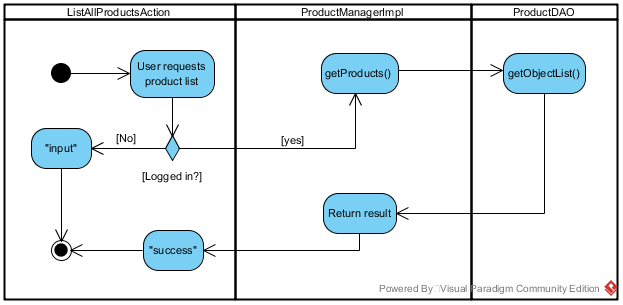
\includegraphics[width=\textwidth]{img/products/list}
		\end{center}
		
		
	For every product in the list, there is the possibility of showing its details. This action is being handled in the class \texttt{ProductDetailsAction}.
	\begin{center}
	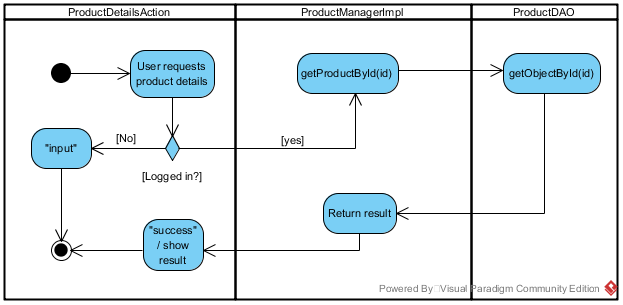
\includegraphics[width=\textwidth]{img/products/details}
	\end{center}
	
	Admins have additional possibilities. They are allowed to add/delete products and create/delete categories that products belong to.
	\begin{center}
	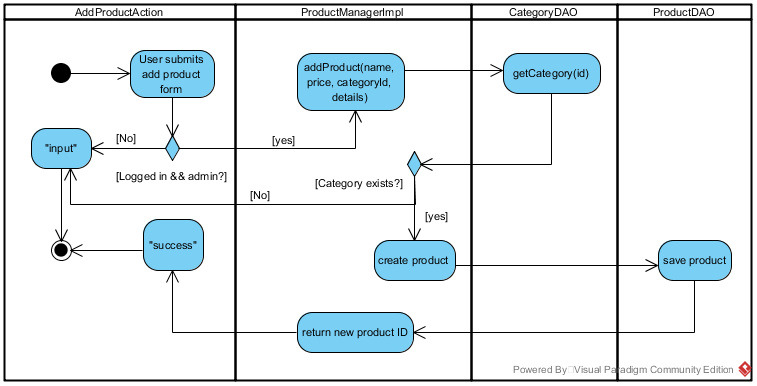
\includegraphics[width=\textwidth]{img/products/createproduct}
	\end{center}
	
	\begin{center}
	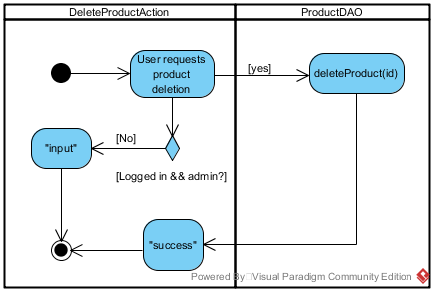
\includegraphics[width=0.7\textwidth]{img/products/deleteproduct}
	\end{center}
	
	\begin{center}
	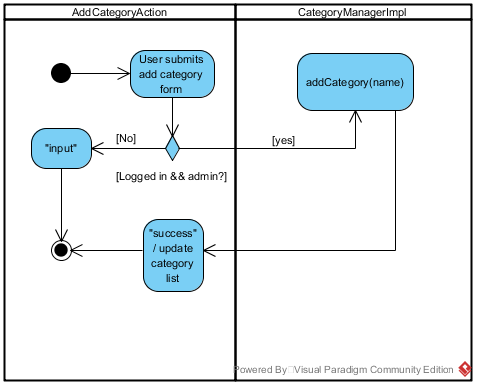
\includegraphics[width=0.7\textwidth]{img/products/addcategory}
	\end{center}
	
	The \texttt{DeleteCategoryAction} works just like the action used to delete a product, but it invokes the \texttt{CategoryDAO} instead of the product access object.
    
    \subsection{Search} % Manu
    \cgraphic{.5}{searchAction-seq}{Search sequence diagram}
    The process of searching for a product with a given criteria is displayed in Figure~\ref{fig:searchAction-seq}. It can only be performed if the user is logged in. If all search fields are left empty, all products of all categories are displayed. If the search text field has a value, the products with the given text search values are looked up. \textbf{Note:} the search is performed as a \textit{like}-search only on the descriptions of the products and not the title. If no search text but and one or more criteria, only the criteria are considered in the search. Furthermore if a criteria is left empty, its minimum or maximum value is considered.
    
   Searching for a product is performed as follows: 
   \begin{enumerate}
   	\item The \texttt{SearchAction} uses the \texttt{ProductManagerImpl} to retrieve products for the given search values.
   	\item The \texttt{ProductManagerImpl} uses the \texttt{ProductDAO} to access the products in database layer.
   	\item The \texttt{ProductDAO} creates and performs the search query using the given search text and criteria for finding the desired products.
   	\item As a last step all categories are loaded for displaying next to the product.
   \end{enumerate}
   
   The class diagram of the SearchAction is displayed below in Figure~\ref{fig:searchAction-class}.
   \cgraphic{.5}{searchAction-class}{SearchAction class diagram}  
   
   \subsection{User management} %Lin
   \cgraphic{.5}{user-management}{User management sequence diagram} 
    The activity diagram for user management is displayed in Figure~\ref{fig:user-management}. The new user can self register with own information. Of cause be able to edit their profile. Only the administrator can create the role (admin, user ..). The administrator can search the user via username or role.
    
    \begin{enumerate}
    	\item The \texttt{registerUser} Action(create user) will check whether the username already exist, if not then create a new user with username, name, lastname, password, role using the UserDAO and RoleDAO.
    	\item The Actor can get a user by username in UserDAO. Equally can get a user or users by RoleLevel(admin, user..) 
    \end{enumerate}
      
\end{document}
